\documentclass{article}

% if you need to pass options to natbib, use, e.g.:
%     \PassOptionsToPackage{numbers, compress}{natbib}
% before loading neurips_2025

% Using default track for workshop submission
\usepackage[final]{neurips_2025}

\workshoptitle{Biosecurity Safeguards for Generative AI}

\usepackage[utf8]{inputenc} % allow utf-8 input
\usepackage[T1]{fontenc}    % use 8-bit T1 fonts
\usepackage{hyperref}       % hyperlinks
\usepackage{url}            % simple URL typesetting
\usepackage{booktabs}       % professional-quality tables
\usepackage{amsfonts}       % blackboard math symbols
\usepackage{nicefrac}       % compact symbols for 1/2, etc.
\usepackage{microtype}      % microtypography
\usepackage{xcolor}         % colors
\usepackage{amsmath}
\usepackage{amssymb}
\usepackage{algorithm}
\usepackage{algorithmic}
\usepackage{graphicx}

\title{Structural Persistence Despite Sequence Redaction:\\ A Biosecurity Evaluation of Protein Language Models}

\author{%
  Petr Simecek\thanks{Corresponding author} \\
  Central European Institute of Technology, Masaryk University\\
  Kamenice 753/5, 625 00 Brno\\
  \texttt{petr.simecek@ceitec.muni.cz} \\
}

\begin{document}

\maketitle

\begin{abstract}
Redacting or deleting portions of sensitive protein sequences is a common practice intended to reduce dual-use risks when publishing or sharing biological data. However, recent advances in generative protein models challenge the effectiveness of this approach. We demonstrate that even after masking up to 85\% of a protein's sequence, state-of-the-art multi-modal models (ESM3) can regenerate sequences that fold into nearly identical three-dimensional structures, preserving complex topological features. Using protein knots as a case study—structures requiring precise spatial arrangements—we show that partial sequence disclosure may not meaningfully reduce the ability of advanced models to reconstruct high-risk proteins. We further demonstrate that models can transform benign proteins into topologically complex variants through iterative modification (31\% success rate). These findings highlight critical vulnerabilities in current biosecurity practices and underscore the need for AI-native defenses that address structural recovery directly. We propose our masking-recovery evaluation framework as a benchmark for assessing biosecurity risks in generative biological AI systems.
\end{abstract}

\section{Introduction}

The rapid advancement of generative AI models for protein design presents a fundamental challenge to biosecurity: how do we prevent the misuse of powerful capabilities while enabling beneficial research? Current biosecurity practices rely heavily on controlling access to complete sequences of potentially dangerous proteins through redaction, database restrictions, and publication guidelines \cite{lewis2020biosecurity_attribution,igsc2024,schmidt2009synthetic,nsabb2007framework}. These approaches assume that partial information significantly impedes reconstruction of functional designs.

We present evidence that this assumption is no longer valid. Using protein knots—complex topological structures found in less than 1\% of known proteins \cite{taylor2000protein}—as a test case, we demonstrate that modern multi-modal protein language models can reconstruct complete, functional structures from heavily redacted sequences. Specifically, we show that ESM3 \cite{hayes2025simulating} can recover knotted protein structures even when 85\% of the original sequence is deleted or obscured.

This ``redaction failure'' phenomenon has immediate implications for biosecurity. Information hazard mitigation strategies based on partial sequence disclosure may provide false security, as access controls that restrict complete sequences but allow partial access could be circumvented. Moreover, publication guidelines that recommend redacting sensitive regions may not prevent reconstruction of dangerous proteins by adversaries with access to modern AI tools.

Recent work has demonstrated the generation of artificial knotted proteins using diffusion models and sequence design tools \cite{klimentova2024unveiling,watson2023novo,dauparas2022robust,alamdari2023protein}, though with extremely low success rates (~0.5\%). Our approach leverages ESM3's guided generation capabilities to achieve dramatically improved recovery rates while highlighting biosecurity implications.

Our contributions are threefold: First, we quantify the robustness of structural features to sequence redaction, establishing that complex topologies persist despite extensive masking. Second, we demonstrate guided generation capabilities that achieve 87\% success in recovering rare structural features, a 170-fold improvement over baseline approaches. Third, we propose a generalizable evaluation framework for assessing reconstruction risks in generative biological AI systems.

\section{Background and Threat Model}

\subsection{Current Biosecurity Practices}

Standard biosecurity measures for sequence data encompass multiple layers of control. DNA synthesis providers screen orders against databases of known pathogens \cite{igsc2024}, while sensitive sequences remain restricted to authorized researchers through controlled access systems. Publications often employ redaction protocols, removing key regions from sequences before public release \cite{nsabb2007framework,schmidt2009synthetic}, and function-based restrictions focus on preventing access to specific functional domains that could be weaponized. These measures collectively assume that incomplete information creates a meaningful barrier to recreating dangerous designs.

\subsection{Capabilities of Modern Protein Models}

Recent protein language models like ESM3 \cite{hayes2025simulating}, AlphaFold3 \cite{abramson2024accurate}, and Boltz \cite{wohlwend2024boltz} integrate multiple modalities in unprecedented ways. These models can predict structure from sequence \cite{lin2023evolutionary}, perform inverse folding to design sequences from structural constraints \cite{hsu2022learning}, execute guided generation with custom objectives \cite{ingraham2019generative,rao2021msa}, and complete masked sequences with high accuracy \cite{rao2019transformer}. These capabilities enable reconstruction pathways that bypass traditional safeguards. The ability to perform guided generation based on scoring functions makes these models particularly suitable for targeting rare protein features that might have dual-use potential.

\subsection{Threat Model}

We consider an adversary who has access to partial sequence information from publications, leaks, or authorized databases, possesses computational resources to run open-source protein models, and seeks to reconstruct functional proteins with specific properties. Critically, we do not assume the adversary has expertise in protein engineering or access to specialized wet-lab facilities for initial design—only for downstream synthesis and testing. This threat model reflects the democratization of AI capabilities, where sophisticated protein design tools are becoming accessible to non-experts.

\section{Methods}

\subsection{Evaluation Framework}

We develop a systematic framework to evaluate structural reconstruction from partial sequences, as detailed in Algorithm \ref{alg:redaction_eval}. This framework systematically tests the ability of modern models to recover functional protein structures from increasingly redacted sequences.

\begin{algorithm}[h]
   \caption{Redaction Robustness Evaluation}
   \label{alg:redaction_eval}
\begin{algorithmic}
   \STATE {\bfseries Input:} protein sequence $s$, redaction levels $R$, trials $N$
   \STATE {\bfseries Output:} reconstruction success rates
   \FOR{each redaction level $r \in R$}
   \STATE Initialize $success\_count = 0$
   \FOR{$i=1$ {\bfseries to} $N$}
   \STATE Randomly redact $r\%$ of sequence $s$ $\rightarrow$ $s_{redacted}$
   \STATE Generate missing regions using model $\rightarrow$ $s_{recovered}$
   \STATE Predict structure of $s_{recovered}$
   \STATE Evaluate structural similarity to original
   \STATE If similarity $>$ threshold: $success\_count$++
   \ENDFOR
   \STATE Record success rate = $success\_count / N$
   \ENDFOR
\end{algorithmic}
\end{algorithm}

\subsection{Test Case: Protein Knots}

We select protein knots as our test case for several strategic reasons. From a biosecurity perspective, protein knots provide an ideal model system that allows us to study reconstruction capabilities without directly working with dangerous sequences. While knots themselves are not inherently harmful, they share critical properties with potentially dangerous protein features: they require precise spatial arrangements that cannot form by chance \cite{virnau2006intricate}, they are rare in nature (occurring in less than 1\% of proteins), making successful generation non-trivial \cite{taylor2000protein,dabrowski2017topological}, and they have clear binary detection criteria using established algorithms \cite{lua2012pyknot,mishra2012knot}.

Most importantly, protein knots represent a level of structural complexity comparable to functional motifs found in dangerous proteins \cite{orengo1997cath}. They exhibit enhanced stability and unique functional properties \cite{strassler2022tied,king2007identification,soler2013effects}, and their evolutionary conservation across species suggests functional importance \cite{brems2022alphafold,begun2024effect,puri2022elucidation}. This makes them an excellent proxy for studying how an adversary might reconstruct functionally important motifs from partial information, without the ethical concerns of working directly with pathogenic sequences.

\subsection{Model and Generation Protocol}

We employ ESM3-SM, the 1.4B parameter version of ESM3, which is currently the only publicly available variant of this powerful model family. While larger versions (7B and 98B parameters) exist and would likely show even stronger reconstruction capabilities, they remain restricted. Our use of ESM3-SM serves as a conservative lower bound for what will soon be possible when larger models become publicly accessible—a scenario that appears increasingly likely given the rapid democratization of AI capabilities \cite{hayes2025simulating}.

For controlled reconstruction, we implement guided generation following:
\begin{equation}
p(x|c) \propto p(x) \cdot \exp(\lambda \cdot s(x))
\end{equation}
where $s(x)$ is a scoring function for desired structural features and $\lambda$ controls guidance strength. We use the Topoly package with Alexander polynomials for knot detection and scoring. See Figure \ref{fig:generated} for an example of generated knotted protein.

\begin{figure}[h]
\centering
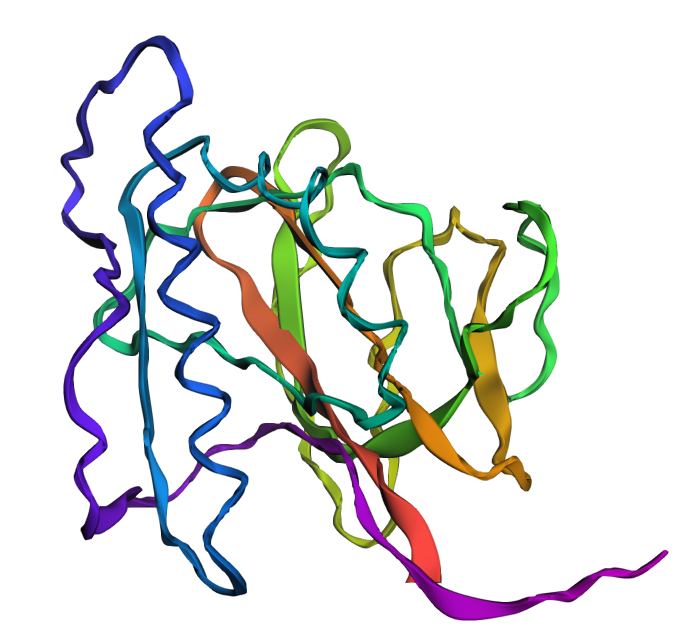
\includegraphics[width=0.45\textwidth]{figures/Figure5b.png}
\caption{Example of a knotted protein generated through ESM3 guided generation. The structure maintains a stable knot topology while exhibiting realistic secondary structure elements.}
\label{fig:generated}
\end{figure}

\subsection{Dataset and Evaluation}

We analyze 1,000 knotted and 4,000 unknotted proteins from publicly available structural databases. For each protein, we apply varying levels of sequence redaction (5\%-95\%), attempt reconstruction using guided generation, verify topological preservation using established knot detection algorithms, and quantify structural similarity using TM-score. This comprehensive evaluation allows us to map the relationship between information retention and reconstruction success.

\section{Results}

\subsection{Structural Features Persist Despite Extensive Redaction}

Our primary finding challenges the effectiveness of sequence redaction as a biosecurity measure. We demonstrate that protein structures, including complex topological features, can be recovered even when the majority of sequence information is withheld.

\begin{figure}[h]
\centering
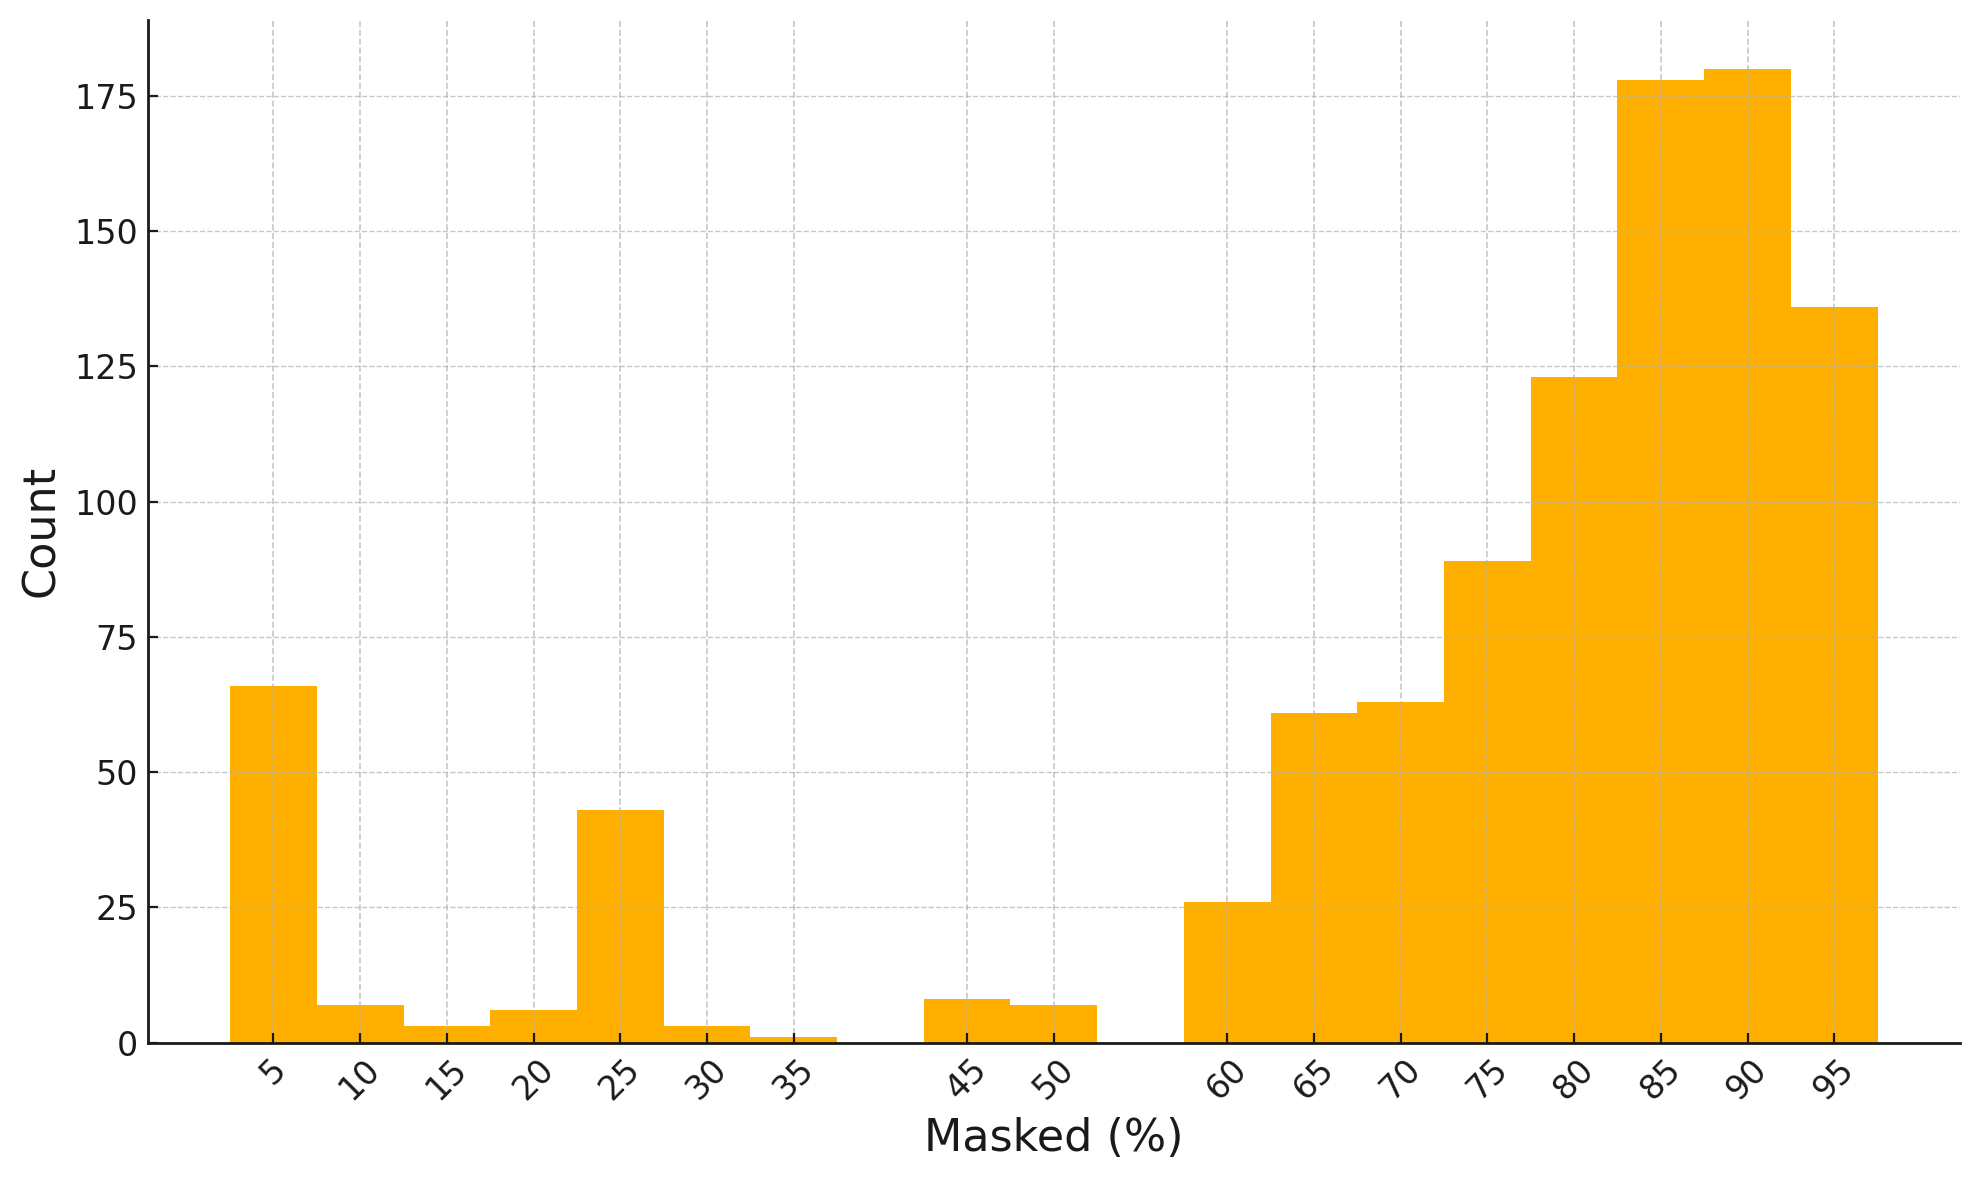
\includegraphics[width=0.8\textwidth]{figures/Fig2hist.png}
\caption{Distribution of minimum sequence retention needed to preserve structural topology. Most proteins maintain their knot structure until 80-85\% of the sequence is redacted, indicating high robustness to information loss.}
\label{fig:redaction_threshold}
\end{figure}

Figure \ref{fig:redaction_threshold} shows that on average, 85\% of a protein sequence must be deleted before the topological structure is lost. This implies that retaining just 15-20\% of a sequence may be sufficient for reconstruction—far less than what typical redaction protocols would remove.

\subsection{Guided Generation Achieves High Recovery Rates}

Using guided generation with structural objectives, we achieve an 87\% success rate in generating knotted proteins from fully masked sequences, representing a 170-fold improvement over the 0.5\% baseline rate observed with unguided generation. Additionally, we demonstrate a 31\% success rate in converting unknotted proteins to knotted variants through iterative modification. These results demonstrate that modern models can be effectively steered toward specific structural outcomes, even extremely rare ones that occur in less than 1\% of natural proteins.

\begin{table}[h]
\caption{Reconstruction success rates at different redaction levels}
\label{tab:reconstruction}
\vskip 0.15in
\begin{center}
\begin{small}
\begin{tabular}{lcc}
\toprule
Redaction Level & Success Rate & Structural Similarity \\
\midrule
25\% & 98\% & 0.95 \\
50\% & 94\% & 0.91 \\
75\% & 87\% & 0.84 \\
85\% & 71\% & 0.76 \\
90\% & 42\% & 0.63 \\
95\% & 18\% & 0.41 \\
\bottomrule
\end{tabular}
\end{small}
\end{center}
\vskip -0.1in
\end{table}

\subsection{Model Embeddings Capture Structural Information}

Training a simple neural network classifier on ESM3 embeddings achieves 93\% accuracy in detecting knotted proteins from sequence alone. This remarkable accuracy indicates that models learn implicit structural representations that capture complex topological features \cite{bepler2019learning,rao2019transformer}. The ability to infer topological features without explicit structural information suggests that partial sequences may contain sufficient signal for reconstruction, even when critical regions appear to be missing.

\subsection{Critical Threshold Behavior}

We observe non-linear degradation in reconstruction success, as shown in Figure \ref{fig:threshold}. Rather than a gradual decline, there exists a critical threshold where reconstruction capability drops sharply. This suggests that a critical amount of sequence information enables reconstruction, and below this threshold, reconstruction fails rapidly. Current redaction practices may unknowingly operate near this critical point, providing a false sense of security.

\begin{figure}[h]
\centering
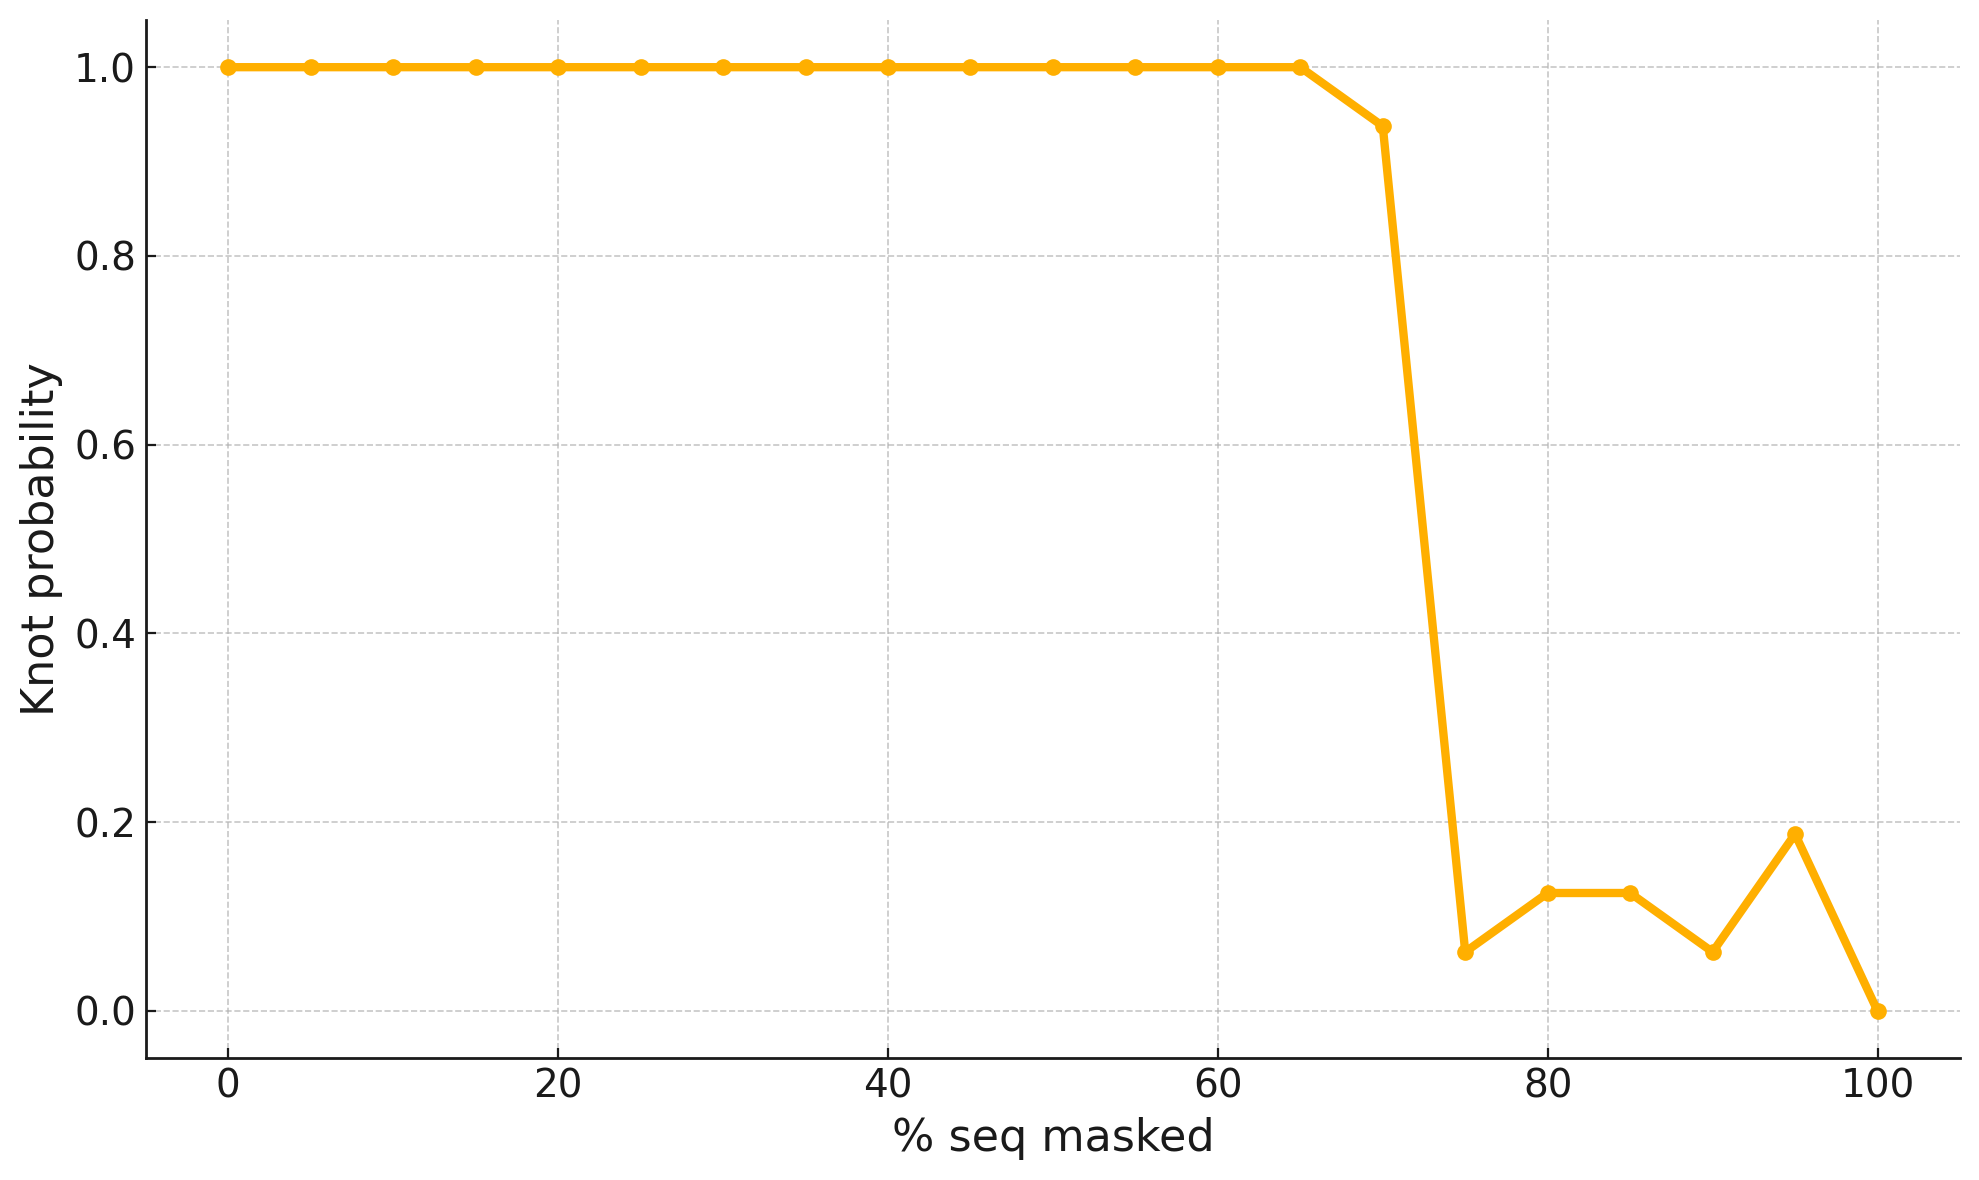
\includegraphics[width=0.8\textwidth]{figures/Fig4actual.png}
\caption{Knot probability after masking for one selected protein. Sharp transition in reconstruction success near the critical redaction threshold, indicating non-linear information requirements.}
\label{fig:threshold}
\end{figure}

\section{Biosecurity Implications}

\subsection{Vulnerability of Current Safeguards}

Our findings reveal three critical vulnerabilities in current biosecurity practices. First, redaction is fundamentally insufficient: removing 50-75\% of a sequence—far more than typically redacted in publications—still allows high-fidelity reconstruction. Second, if complex knots can be recovered from partial information, simpler functional domains such as binding sites or catalytic residues are likely even more robust to redaction. Third, the ability to use guided generation means adversaries don't need complete sequences—just enough information to steer the model toward desired structural outcomes.

\subsection{Implications for Different Threat Scenarios}

The implications extend across multiple threat scenarios. In toxin reconstruction, partial sequences of protein toxins published in scientific literature could be completed to functional designs using guided generation. For virulence factor engineering, key pathogenic domains could be reconstructed from fragments and integrated into novel protein contexts. In the context of immune evasion, antibody escape mutations could be explored even with incomplete structural data, potentially accelerating the development of vaccine-resistant variants \cite{casadevall2014need}.

\subsection{Recommendations for AI-Native Safeguards}

Based on our findings, we recommend a fundamental shift in biosecurity strategy. First, policies should assume that any partial sequence disclosure enables full reconstruction—the traditional assumption that redaction provides meaningful protection is no longer valid. Second, models should incorporate function-based filtering that can detect and refuse to generate sequences with dangerous functions, regardless of input completeness. Third, continuous monitoring of model capabilities for reconstruction from partial information should become a standard component of safety evaluations. Finally, effective biosecurity will require layered defenses that combine model-level safeguards with downstream synthesis screening and anomaly detection systems.

\section{Proposed Evaluation Benchmark}

We propose RedactBench as a standardized evaluation suite for assessing biosecurity risks in generative biological AI systems. This benchmark tests reconstruction capability across different feature types, measures the minimum information needed for successful recovery, evaluates the effectiveness of proposed safeguards, and includes both benign test cases and dual-use relevant features. Key metrics include reconstruction rate at different redaction levels, information threshold for successful recovery, preservation of specific functional motifs, and the ability to bypass different defense mechanisms.

\section{Limitations and Future Work}

Our study has several limitations that should guide future research. We use topological features as a proxy for functional properties, though the relationship between topology and function may vary across protein families. Our experiments were conducted with the smallest publicly available ESM3 model; larger models will likely show even stronger reconstruction capabilities. Additionally, we focus on single-domain proteins, while many dangerous proteins contain multiple domains that might behave differently under redaction.

Future work should extend this evaluation to specific dual-use relevant features, though such research must be conducted with appropriate safeguards and oversight. Testing reconstruction of actual toxin or virulence sequences would provide direct evidence but raises ethical concerns that must be carefully managed. Development and evaluation of AI-native defense mechanisms represents a critical need, as does investigation of reconstruction from non-sequence modalities such as structure fragments or functional descriptions.

\section{Conclusion}

We demonstrate that sequence redaction—a cornerstone of current biosecurity practice—fails to prevent reconstruction of complex protein structures when advanced generative models are available. The ability to recover functional designs from as little as 15-20\% of sequence information fundamentally challenges assumptions about information hazard mitigation in biology.

Our findings underscore the urgent need for new biosecurity approaches that account for AI capabilities. Rather than relying on information restriction alone, we must develop AI-native safeguards that detect and prevent generation of dangerous designs regardless of input completeness. The evaluation framework we present offers a systematic way to assess these risks and test proposed defenses.

As generative models continue to improve, the gap between partial information and functional designs will only narrow. The biosecurity community must adapt quickly, developing new strategies that remain effective even as AI capabilities advance. Our work provides both a warning and a tool for meeting this challenge.

\section*{Acknowledgments}
We thank the anonymous reviewers for their insightful comments. The project was supported by the OPUS LAP program of the Czech Science Foundation, project no. 23-04260L ("Biological code of knots – identification of knotted patterns in biomolecules via AI approach"). Computational resources were provided by the project "e-Infrastruktura CZ" (e-INFRA CZ LM2018140) supported by the Ministry of Education, Youth and Sports of the Czech Republic.

\bibliographystyle{plainnat}
\bibliography{references}

\end{document}